\section{Introduction}
\textit{Ab initio} structure prediction algorithms typically start with a coarse grained search of conformational space through the assembly of previously picked structural fragments. As such, the accuracy of structure prediction is heavily dependent on the similarity of the distribution of fragments for a given position to the target fold \cite{Gront2011-ik}. Thus, the necessary structural information for accurate structure prediction must be encoded in the fragment library for a given target sequence. Additionally, new protein folds are merely the assembly of already known building blocks, such as super-secondary structure motifs \cite{Fernandez-Fuentes2010-iu}. This idea is not novel and has been successfully applied in \gls{nmr} and X-ray crystallography studies \cite{Jones1986-kh,Delaglio2000-pu,Kontaxis2005-bz,Sammito2013-tt}. However, almost all implementations neglect target-specific information generally available to crystallographers through bioinformatics software. This information includes the primary sequence of the target, torsion angle predictions, predicted solvent accessibility or co-evolution information. In theory, all additional information should improve the generation of such fragment libraries by aiding the selection process or cross-validating the identified fragments.

Over the last decade, efforts have been made to improve the precision and coverage of structural fragment libraries used in \textit{ab initio} structure prediction \cite{Shen2013-ag,Li2008-fu,Kalev2011-te,Bhattacharya2016-bp,Wang2017-ox,De_Oliveira2015-ba,Gront2011-ik}. Various different algorithms have been developed to generate static and dynamic fragment libraries. Static fragment libraries are those pre-computed and generally consistent of common super-secondary structure motifs. In comparison, dynamic fragment libraries consist of fragments of variable lengths acknowledging the fragment-dependent optimal length. Most commonly used in \textit{ab initio} structure prediction are dynamic algorithms, such as FLIB \cite{De_Oliveira2015-ba}, NNmake \cite{Gront2011-ik} or HHfrag \cite{Kalev2011-te}. All dynamic-library producing algorithms differ in their definition of ideal fragment lengths, the default number of fragments used per position and they way in which fragments are extracted. However, these algorithms typically share the same additional sequence-based information used to aid the selection of target fragments, which usually includes sequence similarity, three-state secondary structure prediction and torsion angle prediction.

Given that fragment libraries selected to perform \textit{ab initio} structure prediction can contain high quality fragments or super-secondary structure motifs, those fragments must be suitable as \gls{mr} search models. Although the interplay between overall fragment library precision and coverage increases the false positive fragments in a set \cite{Kalev2011-te}, correct identification of true positives should allow for dynamic fragment selection to achieve \gls{mr} structure solution without the overhead of \textit{ab initio} structure prediction. Furthermore, dynamic algorithms could pick fragments of varying lengths, possibly matching co-evolution profiles or other externally obtainable restraints to validate fragments prior to any \gls{mr} attempt. As such, the work in this chapter focuses on exploring this idea using FLIB \cite{De_Oliveira2015-ba}, a dynamic fragment picking algorithm considering co-evolution data to verify fragments during the picking process.

\section{Methods}
\subsection{Target selection}
Four targets were manually selected for this study. The \gls{pdb} identifiers of these targets are: 1aba, 1lo7, 1u06, and 5nfc. The former two are described in \cref{table:methods_dataset_flume}. Target 1u06 is a recently published structure of \textalpha-spectrin SH3 domain (PDB ID: 1kjl in \cref{table:methods_dataset_flume}) with a resolution of 1.49\AA. Target 5nfc is a recently published structure of Galectin-3 (PDB ID: 1kjl in \cref{table:methods_dataset_flume}) with a resolution of 1.59\AA. This resulted in a dataset with similar attributes for each target: crystallographic data resolution of $~1.5$\AA\ with a single molecule in the asymmetric unit, and the target chain length of $<150$ residues.

\subsection{Fragment picking using FLIB}
FLIB \cite{De_Oliveira2015-ba} requires four inputs: the predicted secondary structure, predicted torsion angles, residue-residue contact pair data and a copy of the \gls{pdb}. The secondary structure for each target was predicted using PSIPRED v4.0 \cite{Jones1999-fi} with default parameters. The torsion angles were predicted using SPIDER2 \cite{Heffernan2015-wp} with default parameters, and residue-residue contact pairs using METAPSICOV v1.04 \cite{Jones2015-wp} with default parameters. HHBLITS v2.0.16 \cite{Remmert2011-ze} with database version \texttt{uniprot20\_2016\_02} was used by METAPSICOV to generate the \gls{msa} for contact prediction of each target sequence. BLASTP v2.2.31+ \cite{Altschul1990-nc,Camacho2009-ue} was used by PSIPRED with the UNIPROT database version \texttt{uniref90-2016\_06}. The local copy of the \gls{pdb} for fragment picking was downloaded on August 11, 2016.

Two modifications were made to the default FLIB v1.01 (\url{https://github.com/sauloho/FLIB-Coevo}) protocol. The first focuses on exclusion of fragments with $>90$\% helical content (assigned by DSSP \cite{Frishman1995-ns}). The second modification was to allow fragments with \gls{rmsd} $>10.0$\AA\ to the reference structure to be considered.

Two-hundred fragments were picked per target sequence position. Top-$L$ or $L/2$ contact pairs were selected from both METAPSICOV STAGE 1 and STAGE 2 predictions with a minimum sequence separation of either 6 or 12 residues. Helical fragments were either in- or excluded and only fragments with length between 6 or 12 residues up-to 63 residues considered. Overall, this generated 16 fragment libraries per target.

Each fragment library was then filtered to remove homologs. Hereby, BLASTP and HHPRED \cite{Soding2005-sx} searches were conducted to identify homologous PDB entries. The BLASTP search was performed identically to \cite{De_Oliveira2015-ba}. The HHPRED search parameters were identical to the MPI-Toolkit \cite{Biegert2006-ny} webserver version (\url{https://toolkit.tuebingen.mpg.de/}). Fragments derived from PDB entries identified by BLASTP and HHPRED (probability score of $\geq20.0$) were excluded from the fragment libraries.

All per-target fragments were then binned by their peptide lengths. Subsequently, they were ranked by FLIB scores and \gls{rmsd} values, and the best fragment from each length-dependent bin selected. Fragments of the same template structure consisting of the same region with varying flanking residues were kept, if they were ranked top for each fragment length group. Finally, the coordinates for the selected fragments were extracted and two files created for each, one containing the backbone atoms and the other containing all atoms.

\subsection{\acrlong{mr} in MRBUMP}
The previously extracted fragments were subjected to the \gls{mr} pipeline MRBUMP \cite{Keegan2008-hk}. The latter uses PHASER \cite{McCoy2007-bf} for \gls{mr}, REFMAC5 \cite{Murshudov2011-we} for refinement and SHELXE \cite{Thorn2013-ir} for density modification and main-chain tracing. MRBUMP default parameters were used with exception of the PHASER \gls{rmsd} estimate. Each fragment was subjected to MRBUMP using PHASER \gls{rmsd} values of 0.1, 0.6 and 1.0\AA.

\subsection{Assessment of FLIB fragments}
Fragment torsion angles - predicted by SPIDER2 \cite{Heffernan2015-wp} - were assessed using the \gls{mae}, which evaluates the average absolute difference between the predicted and experimentally determined angles \cite{Heffernan2015-wp}. To account for the periodicity of an angle, the smaller value of the absolute difference $d_i$ and $360-d_i$ was used. The coverage of a fragment library was assessed by the proportion of residues present in at least one fragment in the library. The precision of a fragment library was defined by the fraction of \gls{tp} fragments. All fragments with an \gls{rmsd} of $<1.5$\AA\ were considered \gls{tp} else \gls{fp}. The equation used to calculated the precision score is \cref{eq:methods_precision}. The \gls{rmsd} value, as calculated by FLIB \cite{De_Oliveira2015-ba}, was computed between the aligned residues of the corresponding crystal structure and the fragment. \Gls{mr} success for each search model was solely assessed by SHELXE scores, whereby a \gls{cc} score of $\geq25.0$ combined with an \gls{acl} score of $\geq10.0$ was required.

\section{Results}
\subsection{Precision of FLIB input data}
FLIB requires input data - predicted secondary structure and per-residue torsion angles - alongside the optional co-evolution data corresponding to a given target sequence. The first part of the analysis in this study is the analysis of aformentioned data given that the FLIB fragment picking heavily relies on the individual features in the selection and scoring of each individual fragment \cite{De_Oliveira2015-ba}. Poor data at this stage could lead to poor fragments unsuitable for \gls{mr} trials given that high accuracy, i.e. an low \gls{rmsd} value between the search model and target, is required.

The secondary structure prediction highlighted high precision between each target's prediction and the DSSP-assigned \cite{Frishman1995-ns} secondary structure of the target reference structure (\cref{fig:ample_flib_psipred}). The three targets with \gls{pdb} identifiers 1aba, 1lo7 and 1u06 have secondary structure predictions with a precision of $>72$\%. The fourth target, 5nfc, shows comparatively poor precision of 52.4\%. However, 11 out of 13 secondary structure features are correctly predicted, suggesting successful fragment picking is possible.

\begin{figure}[H]
	\centering
	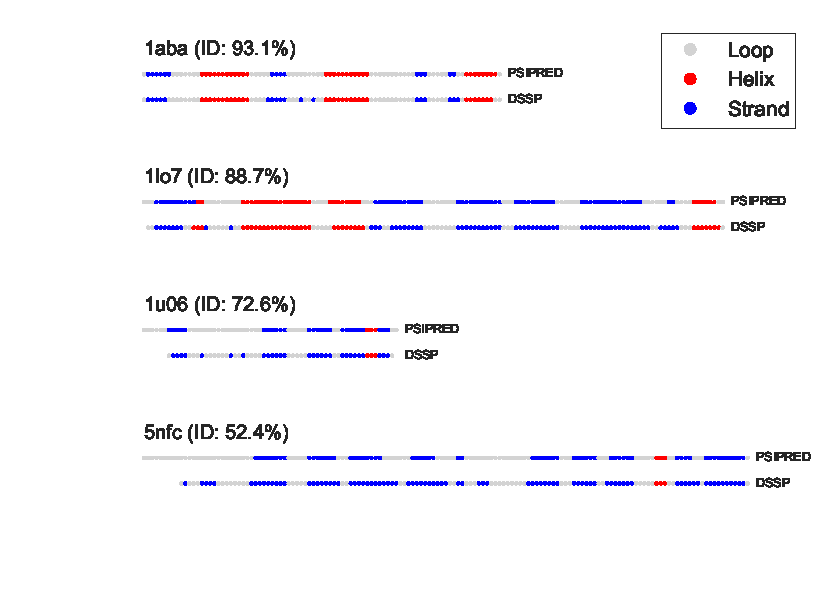
\includegraphics[width=\textwidth]{ample_flib_psipred.pdf}
	\caption[PSIPRED schema for FLIB targets]{Schematic comparison of PSIPRED \cite{Jones1999-fi} secondary structure prediction and DSSP \cite{Frishman1995-ns} assignment. Percentage identity is provided next to each identifier.}
	\label{fig:ample_flib_psipred}
\end{figure}

The contact prediction data for METAPSICOV STAGE 1 and STAGE 2 predictions demonstrate the high precision scores achievable by this algorithm (\cref{table:ample_flib_contact_precision}). In this study, the top contact pairs at cutoffs \textit{L} and \textit{L/2} were provided to the FLIB algorithm. All targets have precision scores for both sets of predictions at both cutoff levels of $>0.6$ (\cref{table:ample_flib_contact_precision}).

\begin{table}[H]
  \small
  \centering
  \caption[Contact prediction summary for FLIB targets]{Precision scores for METAPSICOV \cite{Jones2015-wp} STAGE 1 and STAGE 2 contact predictions. Jaccard index calculated for the same $L$-dependent selection of contact pairs between METAPSICOV STAGE 1 and STAGE 2 predictions.}
  \label{table:ample_flib_contact_precision}
  \begin{tabularx}{\textwidth}{X X X X X X X}
      \hline
	  \multirow{2}{*}{\textbf{Target}} & \multicolumn{3}{c}{\textbf{\textit{L/2} contact pairs}} & \multicolumn{3}{c}{\textbf{\textit{L} contact pairs}} 	\\ \cline{2-7}
	  							&  	Prec\textsubscript{STAGE 1}	& 	Prec\textsubscript{STAGE 2}	& 	Jaccard 	& 	Prec\textsubscript{STAGE 1} 	& 	Prec\textsubscript{STAGE 2} 	& 	Jaccard	 	\\
	  \hline
	  1aba						&	0.884	&	0.884	&	0.303	&	0.713	&	0.759	&	0.513		\\
	  1lo7						&	0.857	&	0.957	&	0.308	&	0.738	&	0.837	&	0.446		\\
	  1u06						&	0.839	&	0.806	&	0.378	&	0.710	&	0.787	&	0.459		\\
	  5nfc						&	0.822	&	0.836	&	0.327	&	0.619	&	0.762	&	0.434		\\ 
	  \hline
  \end{tabularx}
\end{table}

Given the two METAPSICOV contact prediction files, both show localised clusters of contact pairs characteristic for secondary structure features (\cref{fig:ample_flib_cmaps}). These clusters are more populated with contact pairs in METAPSICOV STAGE 2 predictions. This behaviour is to-be-expected given that the second stage in METAPSICOV filters the first for singleton contact pairs whilst enriching the already existing clusters \cite{Jones2015-wp}. Besides the visual analysis, a cluster determination study on each of those contact maps further confirmed a higher singleton frequency in METAPSICOV STAGE 1 predictions. The latter contain on average 9\% more singleton contact pairs and thus a higher degree of noise.

\begin{figure}[H]
	\centering
	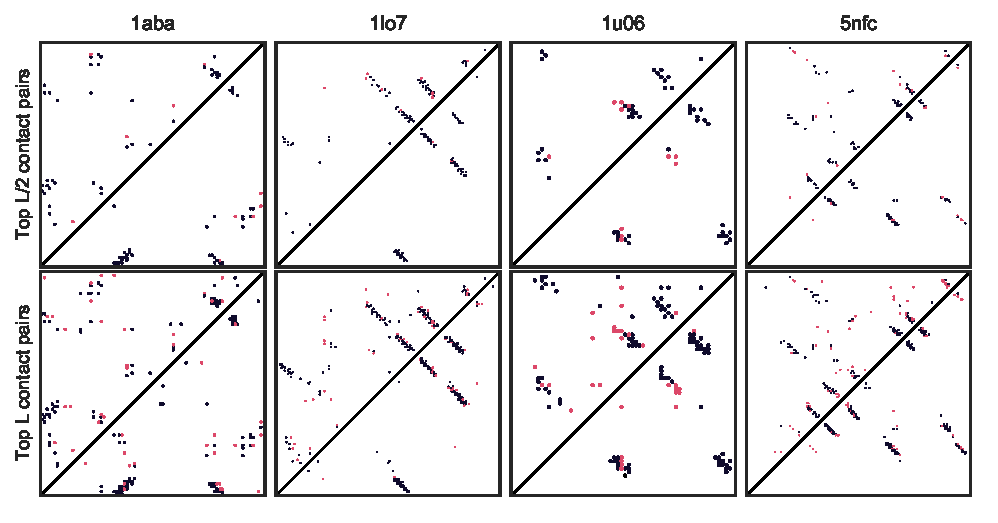
\includegraphics[width=\textwidth]{ample_flib_cmaps.pdf}
	\caption[Contact map comparison for FLIB targets]{Comparison of $L/2$ and $L$ correctly and incorrectly predicted contact pairs for four FLIB targets. Contacts were predicted using METAPSICOV \cite{Jones2015-wp} STAGE 1 (top left) and STAGE 2 (bottom right). True and false positive contact pairs were identified using a 8\AA\ cutoff between C\textalpha\ (C\textbeta\ in case of GLY) atoms of a reference crystal structure. PSIPRED \cite{Jones1999-fi} secondary structure prediction provided along the diagonal.}
	\label{fig:ample_flib_cmaps}
\end{figure}

An analysis of the \gls{mae} of torsion angles between the SPIDER2 \cite{Heffernan2015-wp} prediction and a corresponding reference crystal structure highlights accurate predictions for three of four targets (\cref{fig:ample_flib_spider2}). The largest \gls{mae}\textsubscript{\textphi} across the four target sequences is $24.347^{\circ}$, and the largest \gls{mae}\textsubscript{\textpsi} is $45.459^{\circ}$ (\gls{mae} values for \gls{pdb} entry 1u06). The smallest \gls{mae}\textsubscript{\textphi} is $13.822^{\circ}$ (\gls{pdb} ID: 1aba) and smallest \gls{mae}\textsubscript{\textpsi} is $17.273^{\circ}$ (\gls{pdb}: 1lo7). Segments in sequence space with regular secondary structure, as predicted by PSIPRED \cite{Jones1999-fi}, result primarily in low \gls{mae} values of torsion angles. In contrast, unstructured regions highlight much larger \gls{mae} values indicating the difficulty of predicting these regions. Noticeably, the \gls{mae}\textsubscript{\textpsi} appears to be much larger in those regions than the \gls{mae}\textsubscript{\textphi} for the same residue.

\begin{figure}[H]
	\centering
	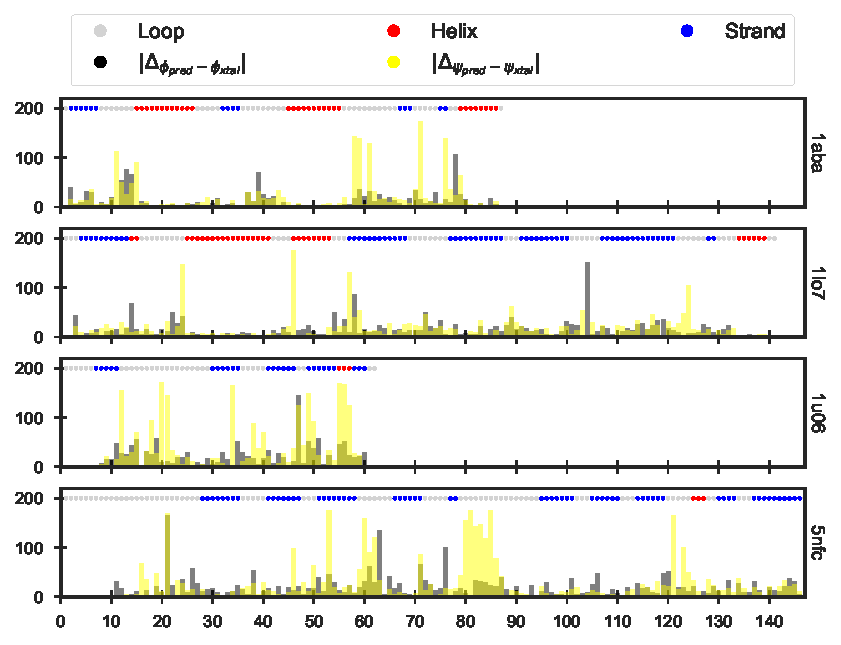
\includegraphics[width=\textwidth]{ample_flib_spider2.pdf}
	\caption[SPIDER2 torsion angle prediction analysis of FLIB targets]{Comparison of \gls{mae} of torsion angles predicted by SPIDER2 and extracted from a corresponding \gls{pdb} structure. PSIPRED \cite{Jones1999-fi} secondary structure prediction provided alongside the \gls{mae} values.}
	\label{fig:ample_flib_spider2}
\end{figure}

\subsection{FLIB fragment picking}
Sixteen FLIB fragment libraries were picked for each protein target in this study. Each fragment library consisted of one permutation given altering input paramaters and contact prediction files.

Across all four targets, the FLIB algorithm selected a total of 8,535,458 fragments (\cref{table:ample_flib_frag_summary}). The fragment libraries show similar statistics across the four protein targets despite the diversity in fold and chain lengths. The mean FLIB score is ~3,200 FLIB score units with a mean \gls{rmsd} of 9.0\AA. Fragments for the alpha-spectrin SH3 domain (\gls{pdb} ID: 1u06) scored the lowest mean FLIB score with 3034 units; however, the same target scored the worst by mean \gls{rmsd} with an average of 9.47\AA. In contrast, fragments picked for the sequence of the bacteriophage T4 glutaredoxin (\gls{pdb} ID: 1aba) achieved the best mean \gls{rmsd} of 7.85\AA\ given the second highest mean FLIB score of 3217 units (\cref{table:ample_flib_frag_summary}).

\begin{table}[H]
  \centering
  \scriptsize
  \caption[FLIB fragment characterics across four protein targets]{Summary of fragment statistics for FLIB libraries selected for four protein targets. Count\textsubscript{H} corresponds to the count of fragments extracted from homologs.}
  \label{table:ample_flib_frag_summary}
  \begin{tabularx}{\textwidth}{X X X X X X X X X}
      \hline
      \multirow{2}{*}{\textbf{Target}} & \multirow{2}{*}{\textbf{Count}} & \multirow{2}{*}{\textbf{Count\textsubscript{H}}} & \multicolumn{3}{c}{\textbf{FLIB score}} & \multicolumn{3}{c}{\textbf{\gls{rmsd}}} \\ \cline{4-9}
      		&			&			& Median 	& Mean 		& Sigma 	& Median 	& Mean 	& Sigma \\
      \hline
      1aba	& 2,091,321	& 45,133		& 3,060.51	& 3,216.87	& 1,405.35	& 7.70	& 7.85	& 3.81	\\
	  1lo7	& 2,497,813	& 23,396		& 3,186.61	& 3,370.99	& 1,496.80	& 9.00	& 9.43	& 4.61	\\
      1u06	& 1,133,517	& 60,159		& 2,901.16	& 3,034.03	& 1,305.64	& 9.51	& 9.47	& 3.94	\\
      5nfc	& 2,812,807	& 48,828		& 2,982.47	& 3,126.60	& 1,316.28	& 8.89	& 9.16	& 4.18	\\
      \hline
      Total	& 8,535,458	& 177516		& 3048.75	& 3207.94	& 1396.74	& 8.68	& 8.96	& 4.25	\\
      \hline
  \end{tabularx}
\end{table}

A split of the per-target fragment libraries into their distinct conditions highlights the improved library quality of certain conditions with regards to the mean FLIB score and \gls{rmsd} (\cref{fig:ample_flib_flibcond}). In particular, top-$L$ (6 residues sequence separation) METAPSICOV STAGE 1 contact predictions yielded the lowest for both metrics across all targets. A comparison of the sequence separation, i.e. using all contact pairs or medium- and long-range ones only, strongly suggests much lower and thus more favourable scores for using short-, medium- and long-range contact pairs. A very similar difference is noticeable for METAPSICOV STAGE 2 contact predictions (\cref{fig:ample_flib_flibcond}). 

\begin{figure}[H]
	\centering
	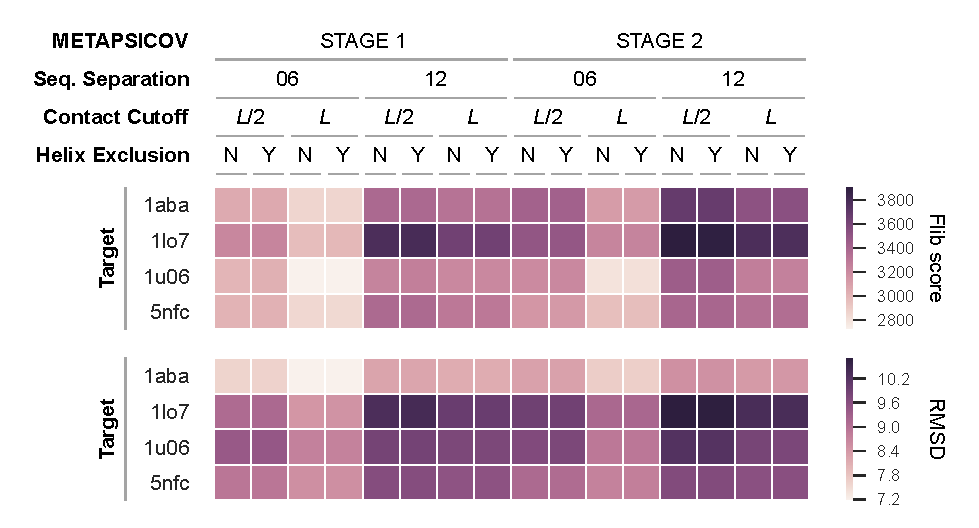
\includegraphics[width=\textwidth]{ample_flib_flibcond.pdf}
	\caption[FLIB fragment library comparison]{FLIB fragment library comparison for four targets highlighting the differences in mean FLIB score and \gls{rmsd} by starting with different subsets of contact predictions. $L$ refers to the number of residues per target sequence. $Y$ refers to idealised \textalpha-helical fragment exclusion during fragment picking; $N$ refers to treating those fragments like all others.}
	\label{fig:ample_flib_flibcond}
\end{figure}

An analysis of the coverage of the target sequence with respect to each picking strategy further demonstrates the benefits of starting with METAPSICOV STAGE 1, i.e. noisier, contact predictions (\cref{fig:ample_flib_fragtps}). Coverage is more evenly spread across the target sequences compared to missing regions especially for target 1lo7 with METAPSICOV STAGE 2 predictions. Noticeably, none of the picking strategies yielded any fragments for the C-terminus of 5nfc (\cref{fig:ample_flib_fragtps}). Furthermore, an analysis of the precision of fragments in each library strongly supports the benefits of starting with top-$L$ (6 residues sequence separation) METAPSICOV STAGE 1 contact pairs. Across all four targets, the coverage of correct fragments (as assessed with a \gls{rmsd} $<1.5$\AA\ to the reference structure) is highest for this condition. This is of particular importance for targets 1u06 and 5nfc, for which most strategies picked very few to no correct fragments. Lastly, correct fragments co-localise with high-density contact regions, further highlighting the importance of this additional source of information. 

The exclusion of idealised \textalpha-helical fragments did not affect the overall FLIB score or \gls{rmsd} greatly ($max \Delta_{FLIB}=25.68; max \Delta_{RMSD}=0.06$).
 
\begin{figure}[H]
	\centering
	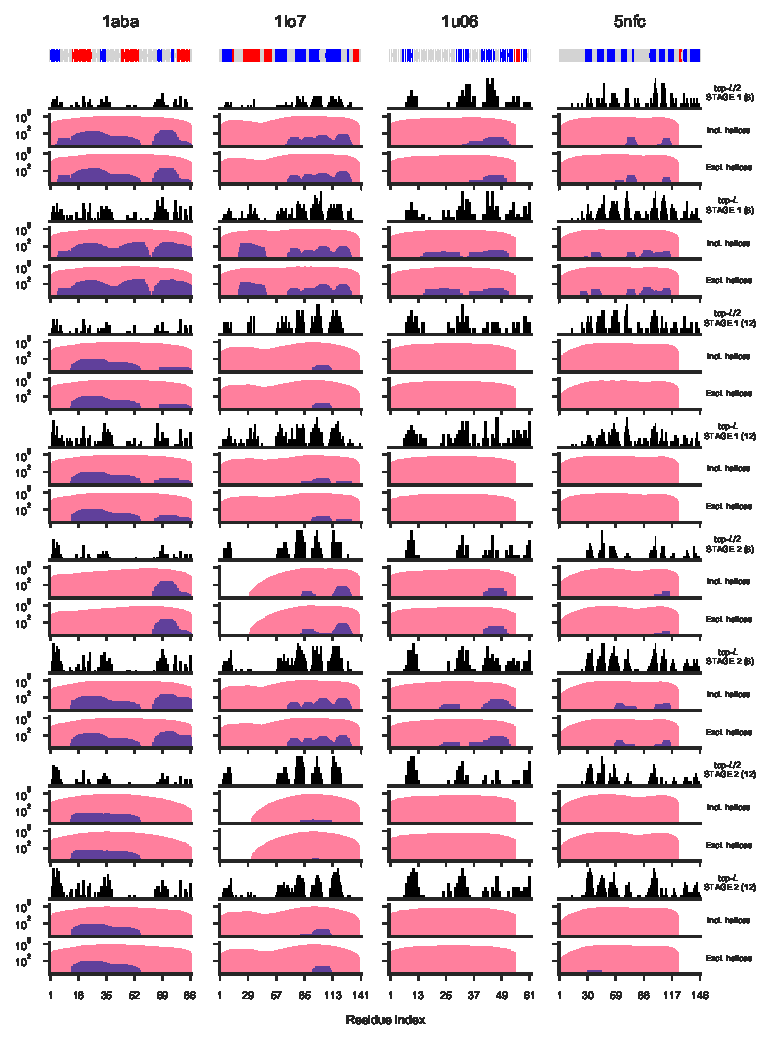
\includegraphics[width=\textwidth]{ample_flib_fragtps.pdf}
	\caption[Coverage and precision of Flib fragment libraries]{Summary of the coverage and precision of FLIB fragment libraries according to their target sequence. The coverage of all fragments with respect to their target-aligned sequence register are shown in red bars, and fragments with \gls{rmsd} $<1.5$\AA\ to the reference structure in blue. The predicted secondary structure of each target sequence is given at the top: \textalpha-helices (red), \textbeta-strands (blue), and loops (gray). Contact prediction information is illustrated using black bars. The fragment frequency is shown using a log-scale.}
	\label{fig:ample_flib_fragtps}
\end{figure}

\subsection{FLIB fragment selection for \acrlong{mr}}
One of the most important aspects of bypassing \textit{ab initio} structure prediction and using the relevant fragments directly as \gls{mr} search models is the selection of the fragments with the highest similarity between fragment and target structure. The FLIB score - a cumulative metric judging the quality of a fragment - is the most obvious feature; however, it is unknown to-date whether a correlation between the FLIB score and the fragment \gls{rmsd} exists. Taking all non-homologous fragments in this study, a first attempt was made to identify a correlation between a fragment's FLIB score and \gls{rmsd}. The results presented here indicate towards a positive correlation between the FLIB score and the corresponding fragment \gls{rmsd} for almost all fragments across the different target fragment libraries (\cref{fig:ample_flib_flibrelat}). However, a small fraction of fragments appear as outliers, not fitting the correlation of lower FLIB scores corresponding to lower \gls{rmsd} values. On average, 0.2\% of fragments per library are contained in this outlier set.

\begin{figure}[H]
	\centering
	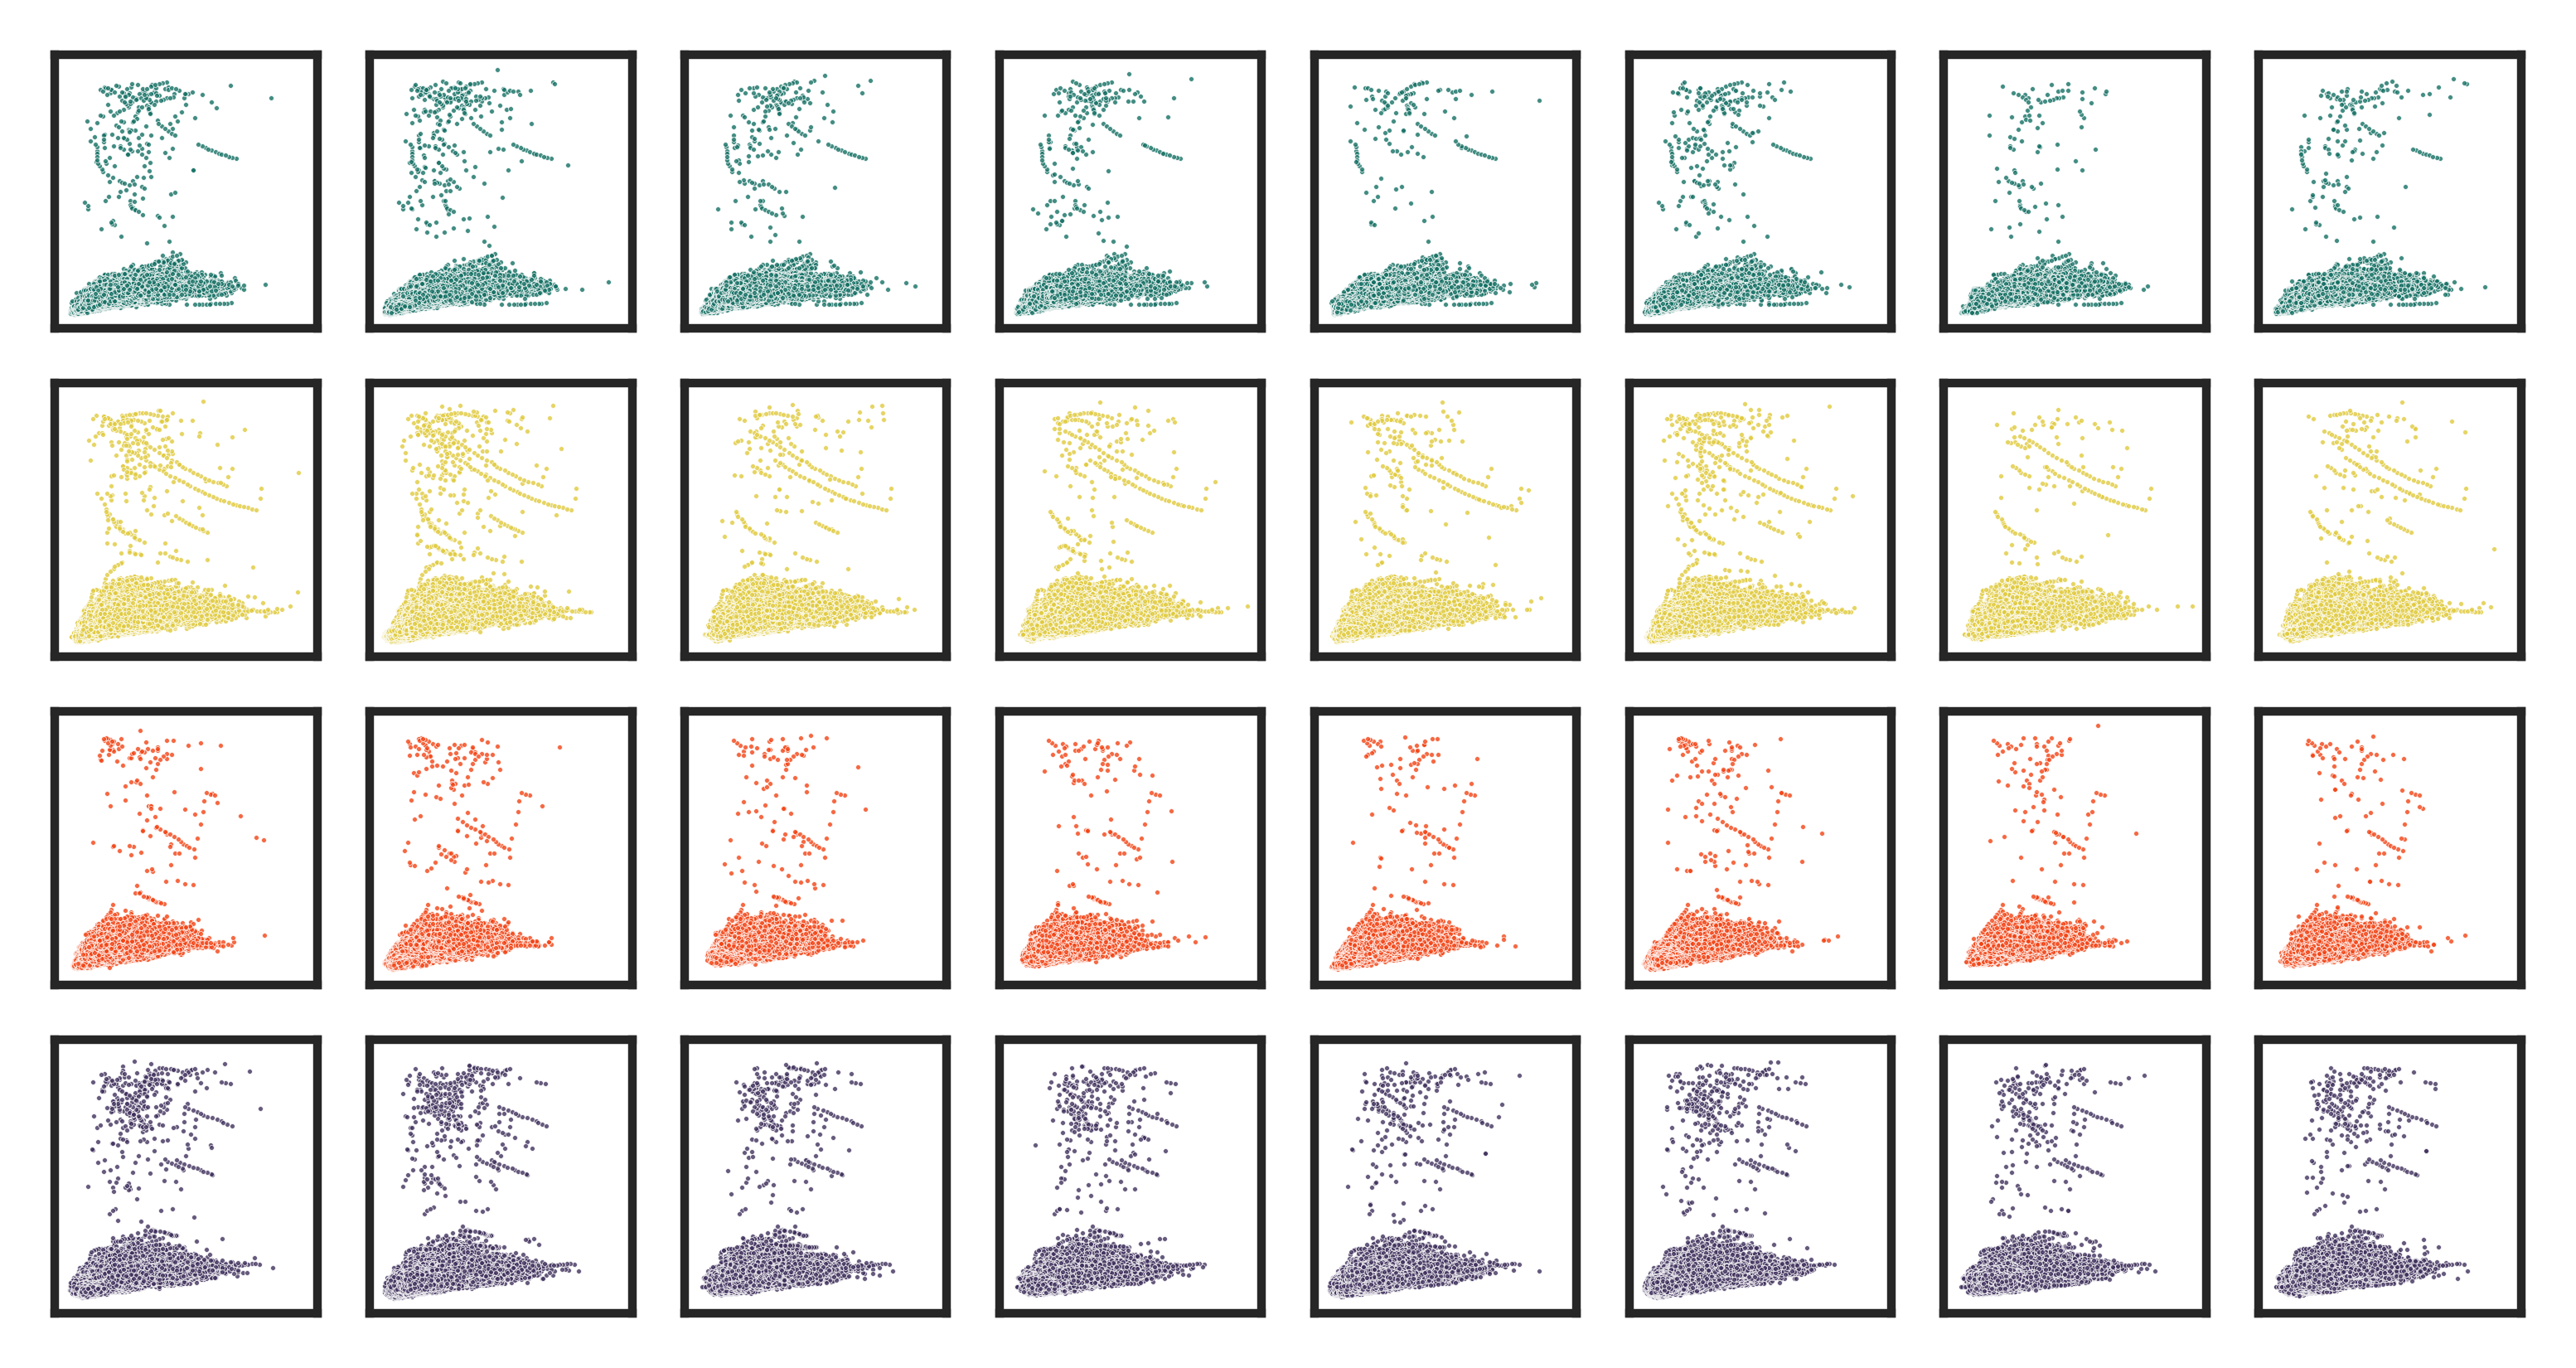
\includegraphics[width=\textwidth]{ample_flib_flibrelat.png}
	\caption[Correlation analysis for FLIB score and \gls{rmsd}]{Scatterplot highlighting the positive correlation between fragment FLIB scores (x-axes) and \gls{rmsd} values (y-axes). Four targets are illustrated: 1aba (green), 1lo7 (yellow), 1u06 (orange), and 5nfc (purple). Each column represents a different fragment picking strategy, and no fragment illustrated corresponds to an idealised \textalpha-helix.}
	\label{fig:ample_flib_flibrelat}
\end{figure}

An analysis of the outliers for characteristics that would allow for their exclusion showed the randomness in their occurrence. These fragments contain all secondary structure types, span the entire target sequence and range all peptide lengths. Furthermore, they occur in all fragment libraries, irrelevant of their original picking strategy. The only characteristic setting these outlier fragments apart from the remaining set is a \gls{rmsd} value of $>30$\AA. Nevertheless, it appears that these outlier fragments with unusually high \gls{rmsd} values are not to be included in the final fragment search model set, given that their overall FLIB\textsubscript{min} score is 796 units, which is one order of magnitude more than the overall minimum for the remaining fragments.

\begin{figure}[H]
	\centering
	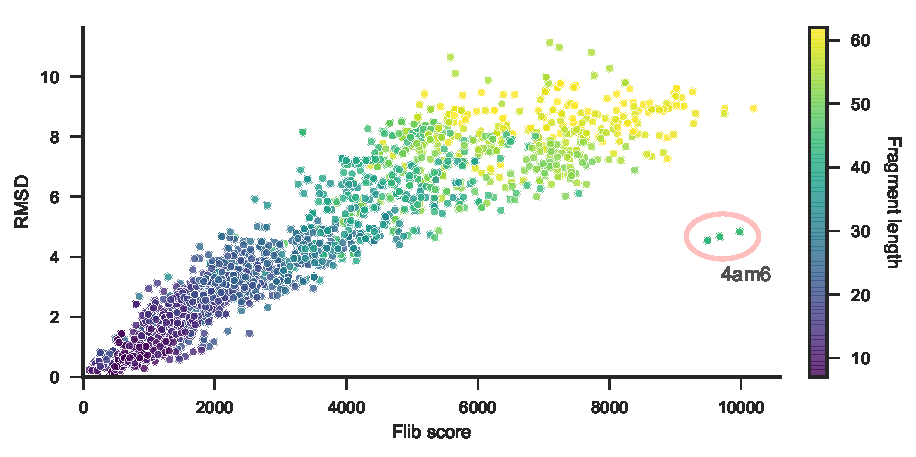
\includegraphics[width=\textwidth]{ample_flib_finalrelat.pdf}
	\caption[Correlation analysis for final FLIB \gls{mr} fragments]{Scatterplot highlighting the positive correlation between fragment FLIB scores and \gls{rmsd} values. The plot contains all fragments independent of target or picking strategy. The colour of each scatter point illustrates the fragment length. Outlier fragments derived from \gls{pdb} entry 4am6 are highlighted.}
	\label{fig:ample_flib_finalrelat}
\end{figure}

A closer inspection of the fragment metrics in the final \gls{mr} set further supports the positively linear relationship between a fragment's FLIB score and \gls{rmsd} (\cref{fig:ample_flib_finalrelat}). Thus, the FLIB score can be related to the similarity of a fragment with the target structure. Furthermore, the size of the fragments also positively correlates with the the FLIB scores and \gls{rmsd}. Longer fragments - with higher proportions of dissimilarity between fragment and target - show higher FLIB scores and \gls{rmsd} values (\cref{fig:ample_flib_finalrelat}). Noticeably, a cluster of large fragments with some of the highest FLIB scores in the set show a reasonable similarity to their target structure (\cref{fig:ample_flib_finalrelat}). All fragments in this cluster were picked for the bacteriophage T4 glutaredoxin sequence (\gls{pdb} ID: 1aba) and extracted from the same region of the crystal structure of the actin-related protein ARP8 (\gls{pdb} ID: 4am6). In comparison, some smaller fragments with peptide lengths $<50$ residues and lower FLIB scores of $<3000$ show the highest \gls{rmsd} values in the final set.

One further unique aspect of this study compared to other fragment-\gls{mr} approaches is the use of residue-residue contact information to score fragments during picking, preferring those which satisfy at least one contact pair. In the final set 39\% of all fragments satisfy at least one, 26\% at least two and 20\% at least three contact pairs. Across the four targets, 50\% of fragments selected for 4-hydroxybenzoyl CoA thioesterase (\gls{pdb} ID: 1lo7) (\cref{fig:ample_flib_consatis}). The fragments selected for the \textalpha-spectrin SH3 domain (\gls{pdb} ID: 1u06) show the lowest contact pair satisfaction with 28\%.

\begin{figure}[H]
	\centering
	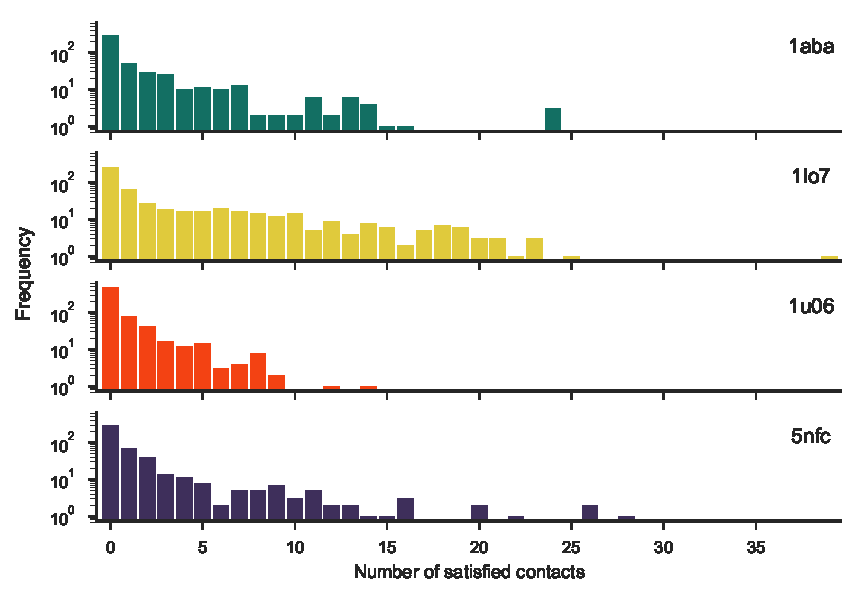
\includegraphics[width=\textwidth]{ample_flib_consatis.pdf}
	\caption[Contact satisfaction of FLIB-derived fragments]{Distribution of contact satisfaction given all \gls{mr} fragments per target.}
	\label{fig:ample_flib_consatis}
\end{figure}

% Lastly, FLIB fragments in the final set comprise a diverse set of short super-secondary structure motifs to small substructures (\cref{fig:ample_flib_search_models}). Depending on the target, the predominant secondary structure  type in the fragment search models changes. Importantly, not a single super-secondary structure motif dominates the set, increasing the sampling diversity to be undertaken during \gls{mr}.

% \begin{figure}[H]
% 	\centering
% 	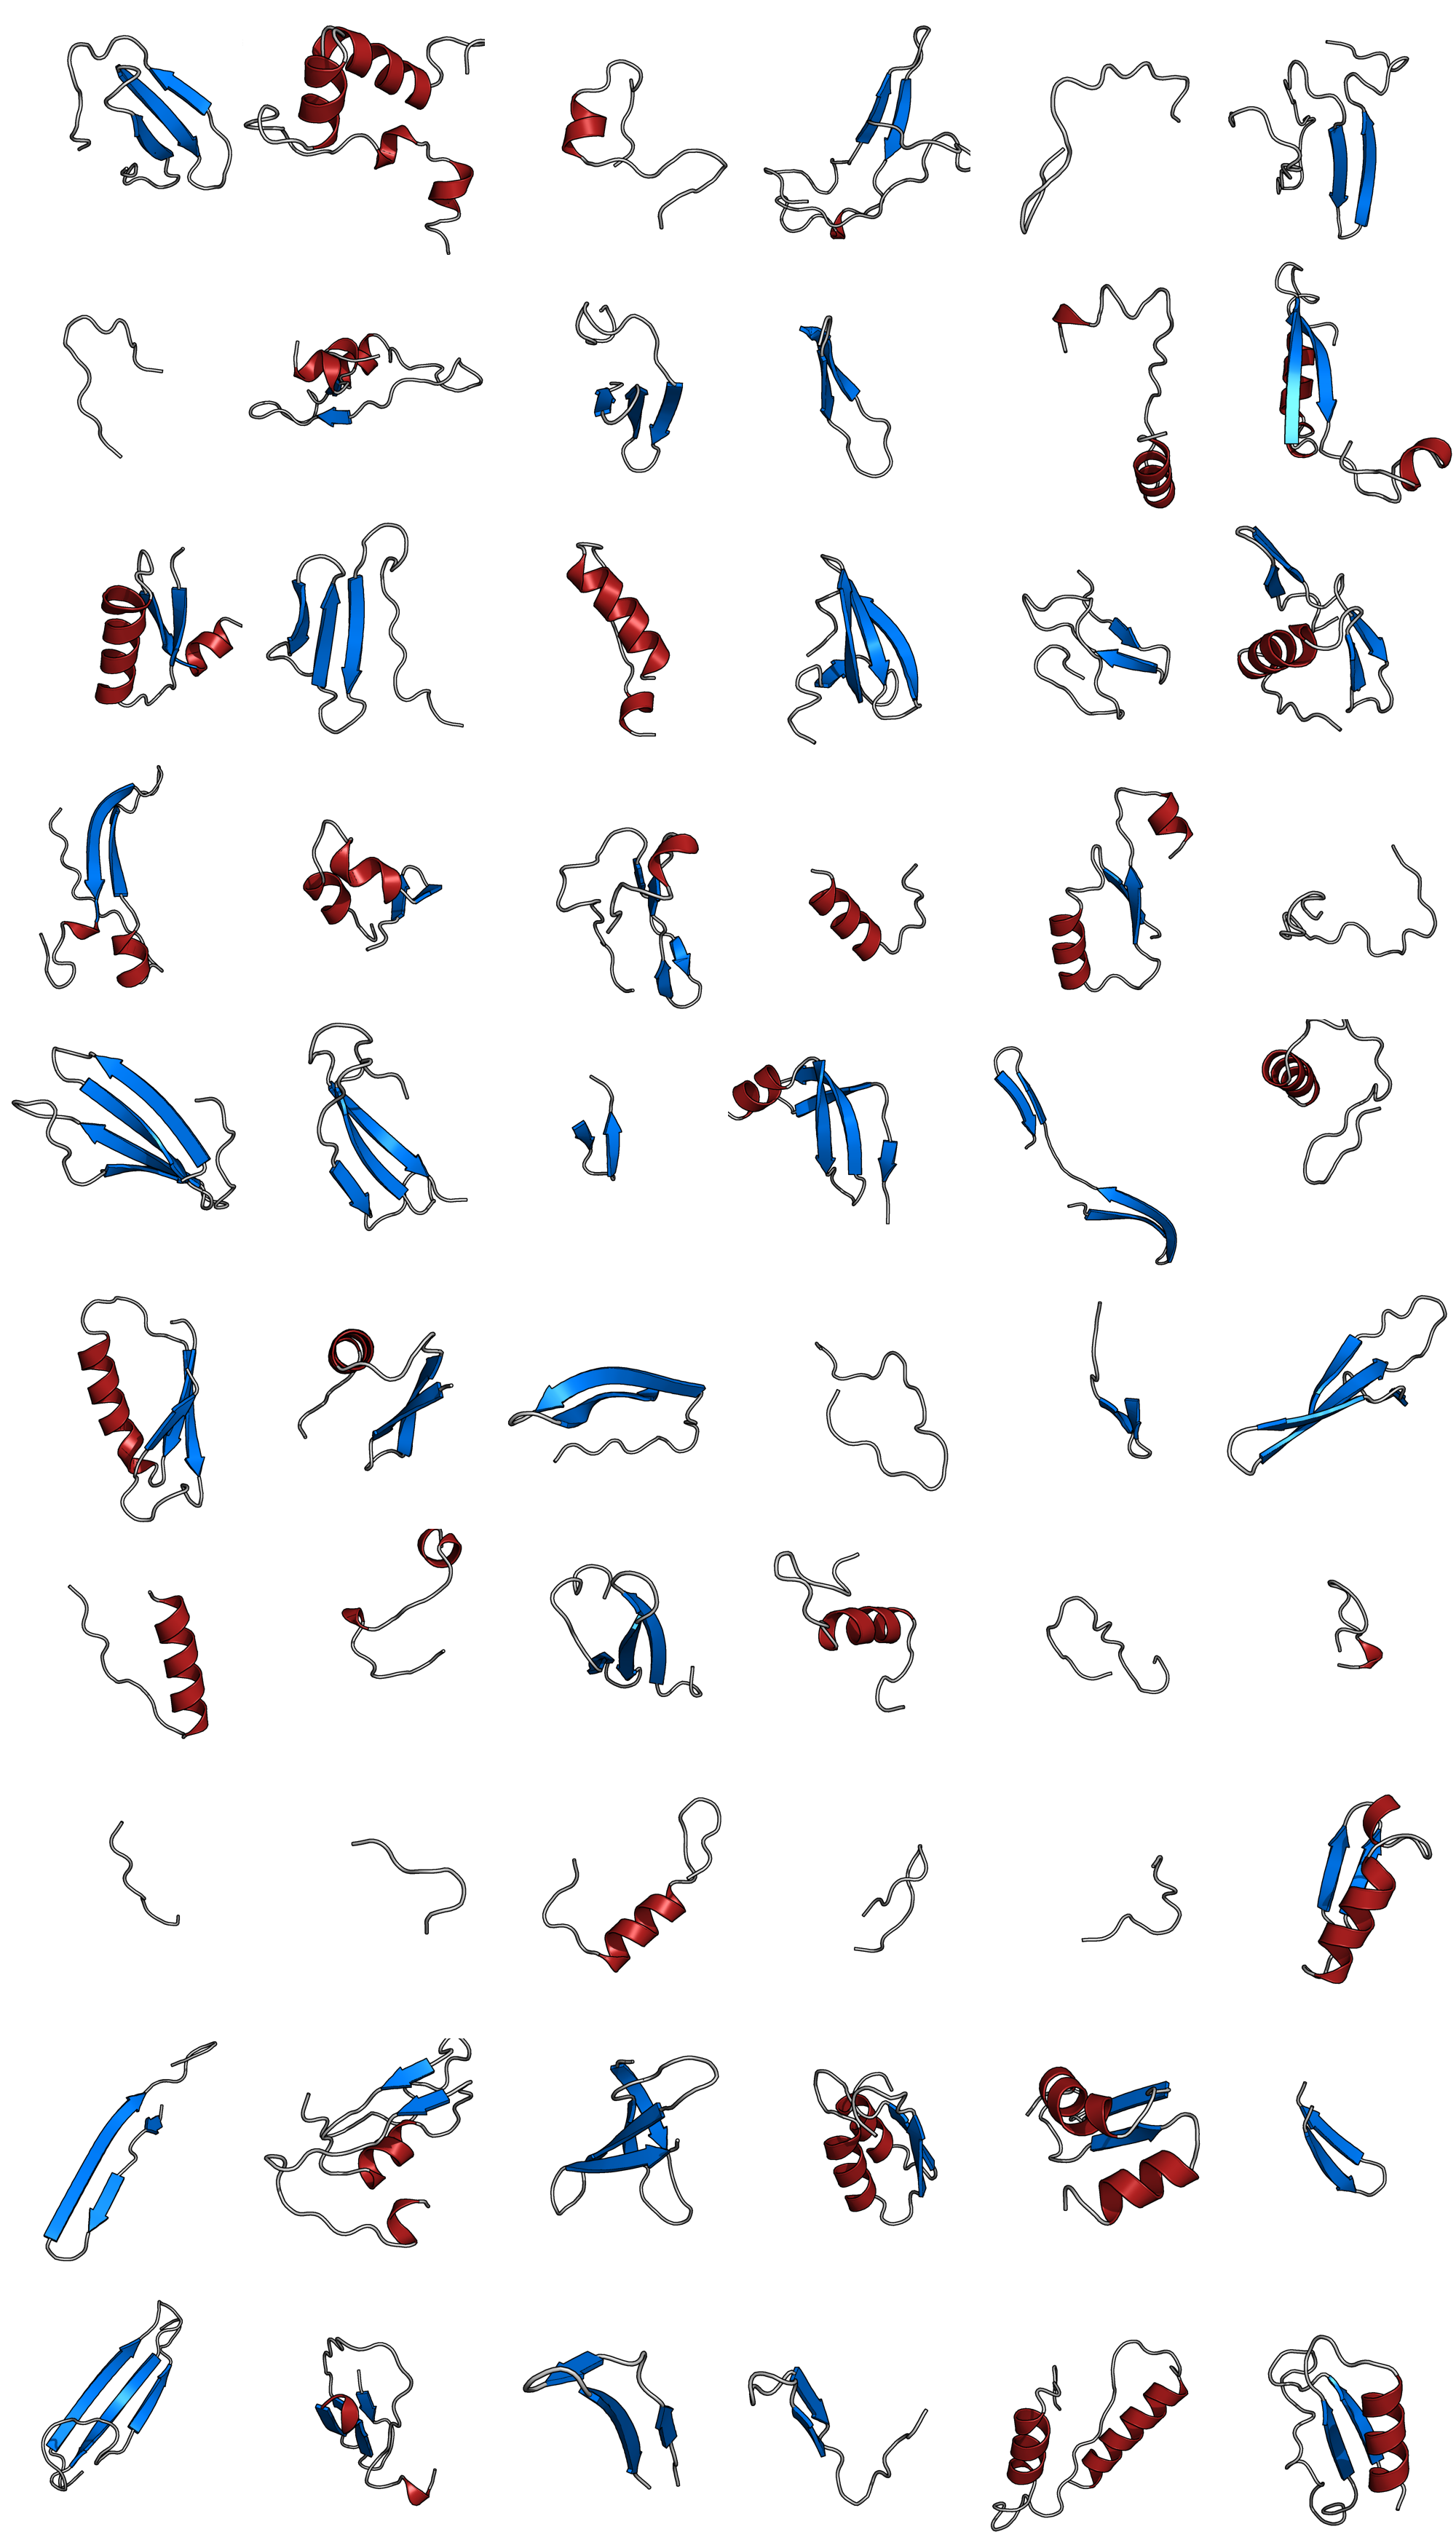
\includegraphics[height=\textheight]{ample_flib_search_models1.png}
% \end{figure}

% \begin{figure}[H]\ContinuedFloat
% 	\centering
% 	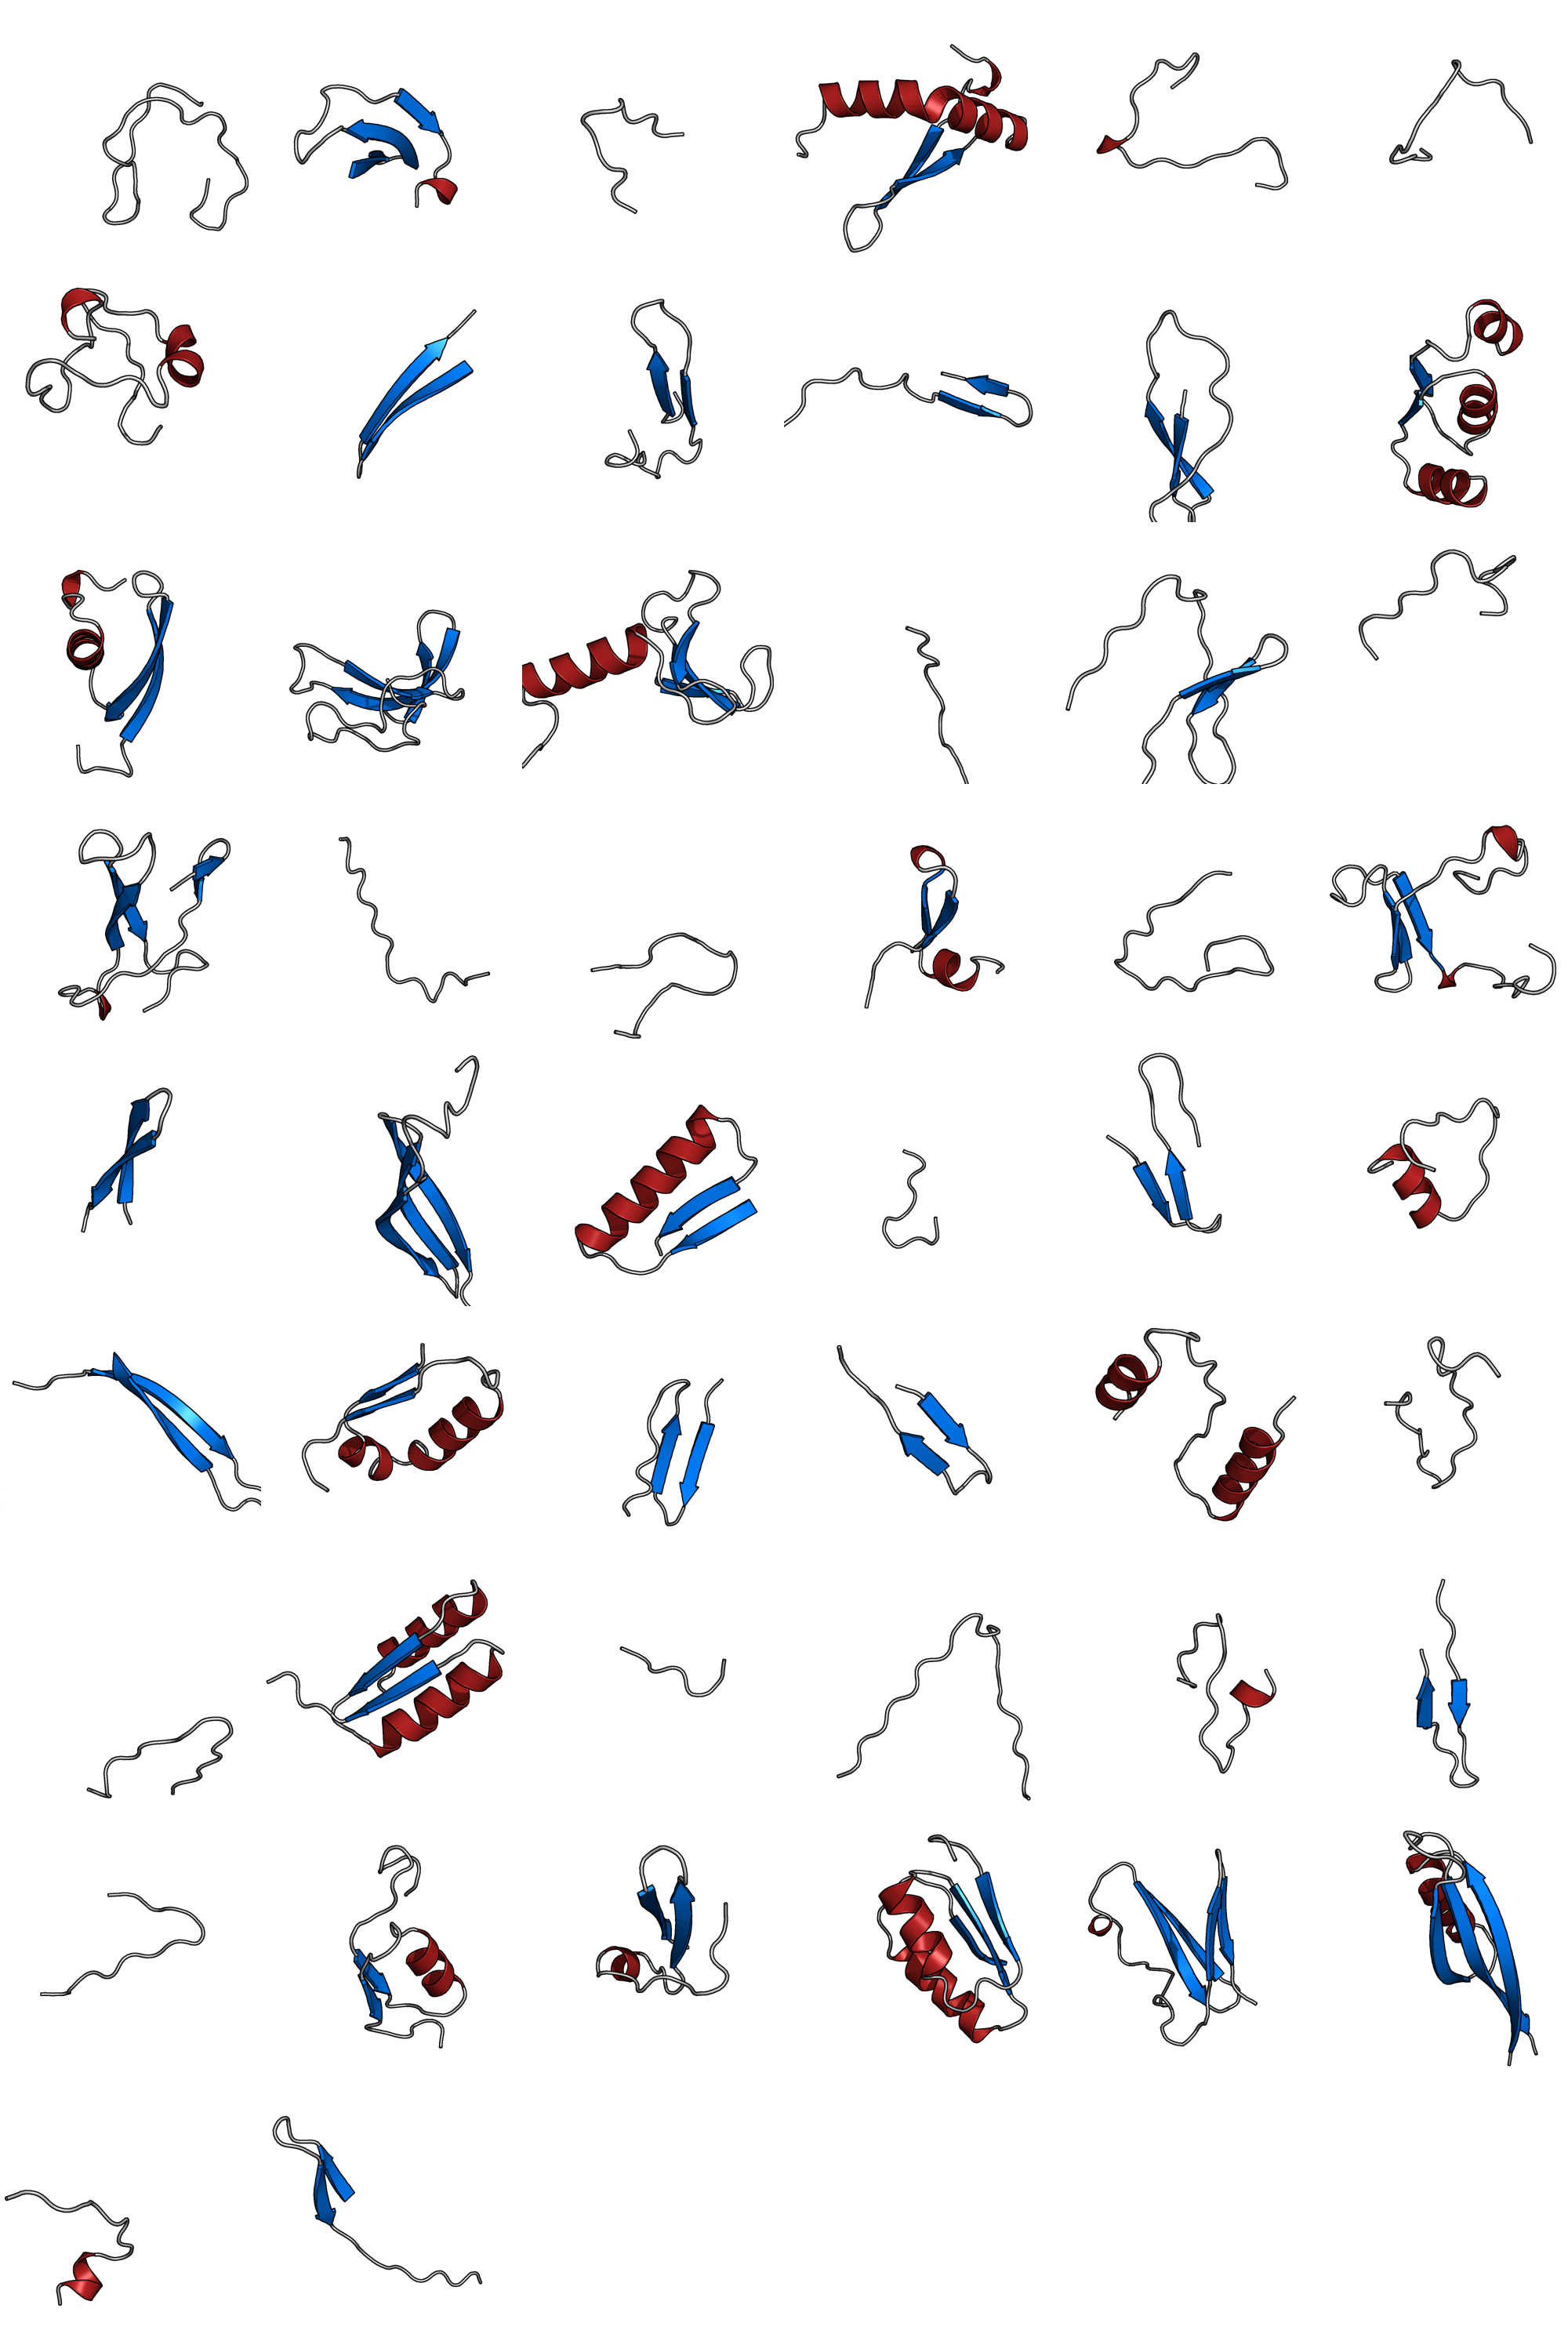
\includegraphics[width=\textwidth]{ample_flib_search_models2.png}
% 	\caption[Fragment search models derived from FLIB]{Non-redundant sample of fragment search models selected for four different protein targets.}
% 	\label{fig:ample_flib_search_models}
% \end{figure}

\subsection{\acrlong{mr} using FLIB fragments}
FLIB fragments picked for four target sequences using a variety of FLIB input options generated $>6,500$ fragments, which were subjected to the \gls{mr} pipeline MRBUMP with their corresponding target experimental data. Given that each fragment was trialled with two different side-chain treatments and 3 different PHASER \gls{rmsd} values, a total of 39,432 \gls{mr} attempts were made across four target structures. Out of nearly 40,000 \gls{mr} attempts 598 led to the structure solutions of two targets, namely the T4 glutaredoxin (\gls{pdb} ID: 1aba) and \textalpha-spectrin SH3 domain (\gls{pdb} ID: 1u06) (\cref{fig:ample_flib_mrsummary}).

\begin{figure}[H]
	\centering
	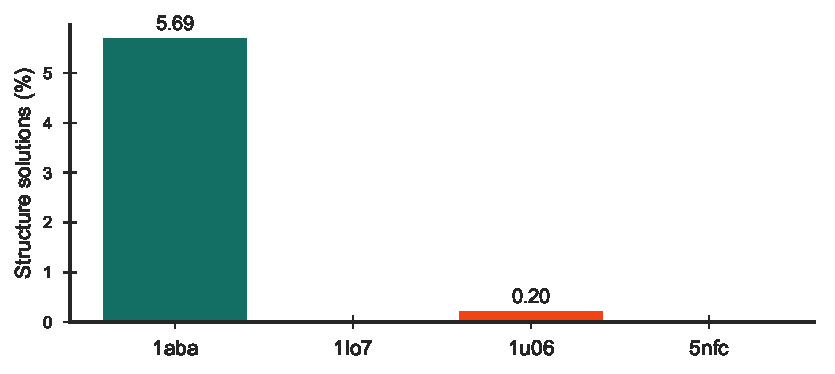
\includegraphics[width=\textwidth]{ample_flib_mrsummary.pdf}
	\caption[MR structure solutions by FLIB target]{Distribution of structure solutions by FLIB target. All \gls{mr} attempts total to 39,432, out of which 598 are structure solutions. Values above each bar indicates percentage search models successful out of the corresponding set.}
	\label{fig:ample_flib_mrsummary}
\end{figure}

A division of FLIB-fragment search models by their respective origin libraries provides further evidence that METAPSICOV STAGE 1 contact predictions allows for the selection of the most accurate fragments (\cref{fig:ample_flib_flibcond}), which directly translates into the structure solution count (\cref{fig:ample_flib_flibcondmr}). Furthermore, this division also highlights and supports the quality of fragment libraries picked with top-$L$ (min. 6 residues sequence separation) METAPSICOV STAGE 1 predictions. Trialling the optimal fragment picking strategy with and without helical fragments ($>90$\%-helical content assigned using DSSP) resulted in the library without to outperform the other (\cref{fig:ample_flib_flibcondmr}, 3rd and 4th bars). 

\begin{figure}[H]
	\centering
	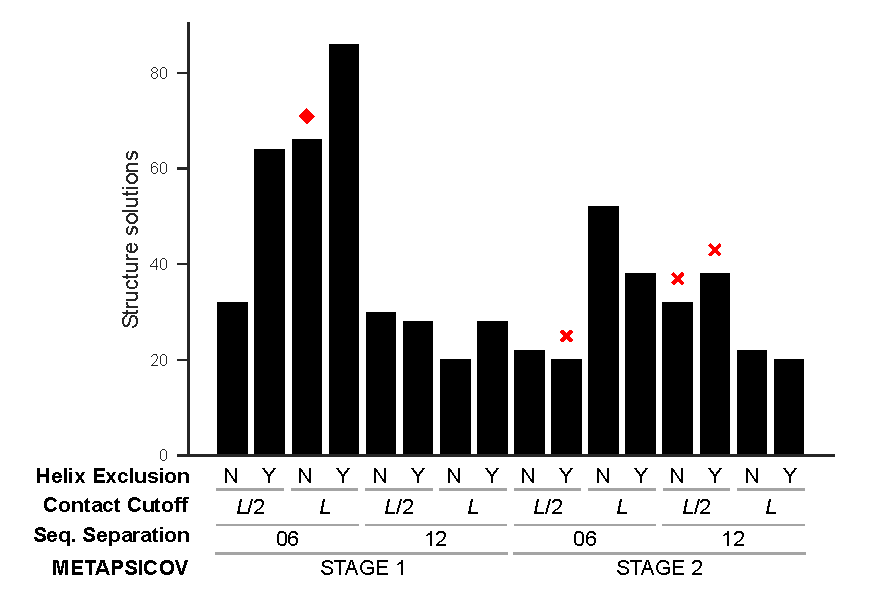
\includegraphics[width=\textwidth]{ample_flib_flibcondmr.pdf}
	\caption[MR structure solutions by FLIB library]{Distribution of structure solutions by FLIB library configuration. The star above the third bar marks this bar as the most optimal by \gls{rmsd} and FLIB score after fragment picking.}
	\label{fig:ample_flib_flibcondmr}
\end{figure}

An analysis of the binned results by fragment-ranking, side-chain treatment or PHASER \gls{rmsd} value confirms the expected outcome that \gls{rmsd}-sorted fragments result in more structure solutions than the FLIB-sorted counterparts (\cref{fig:ample_flib_mrbyconfig}). Nearly two-thirds of the trialled fragments were the best in their libraries when grouped by lengths and sorted by their \gls{rmsd} values. However, the structure of \textalpha-spectrin SH3 domain (\gls{pdb} ID: 1u06) was only solved with FLIB-ranked fragments. A further separation of the successful \gls{mr} fragments reveals no difference between the two side-chain treatments with identical numbers of successful fragment search model attempts. Furthermore, a separation of attempts by PHASER input \gls{rmsd} value suggests a value of 0.1 to be the most favourable.

\begin{figure}[H]
	\centering
	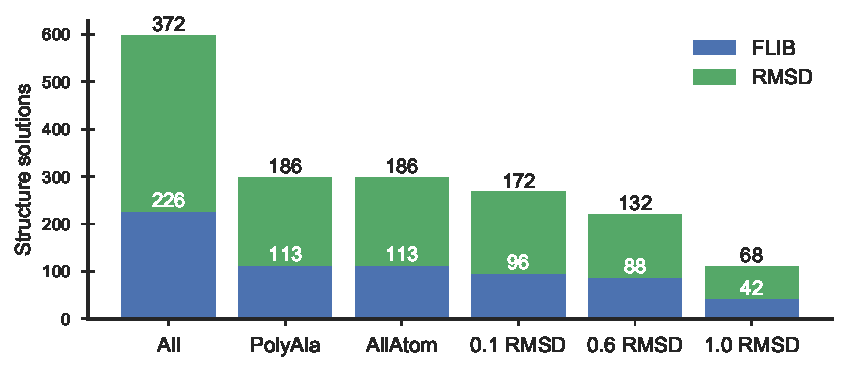
\includegraphics[width=\textwidth]{ample_flib_mrbyconfig.pdf}
	\caption[MR structure solutions by input parameters]{Distribution of structure solutions by fragment and MRBUMP configuration.}
	\label{fig:ample_flib_mrbyconfig}
\end{figure}

In \gls{mr}, the correct placement of very small structural fragment may not always be detectable by the output metrics of underlying software. In benchmarking exercises, the \gls{rio} metric has shown to be a very useful and powerful metric to detect such situations \cite{Thomas2015-ag,Simkovic2016-jx,Thomas2017-lq}. Given that the peptide lengths of FLIB fragments in this study range from 6 to 63 residues, the \gls{rio} score is most suitable in validating the correct placement of FLIB-fragment search models. Indeed, all fragments with SHELXE \gls{cc} $\geq25$ and \gls{acl} $\geq10$ contain at least 3 correctly placed C\textalpha\ atoms (i.e. a \gls{rio} score $\geq3$). Furthermore, the\gls{rio} metric indicates that more than 1,000 fragments have C\textalpha\ atoms placed within 1.5\AA\ of any atom in the target structure. However, only 4 residues are on average placed correctly, which is not enough to achieve structure solution (\cref{fig:ample_flib_mrrionorm}). All successful FLIB fragments have a minimum model- and target-normalised \gls{rio} scores of 29.7\% and 9.2\% (\cref{fig:ample_flib_mrrionorm}, green markers). 

\begin{figure}[H]
	\centering
	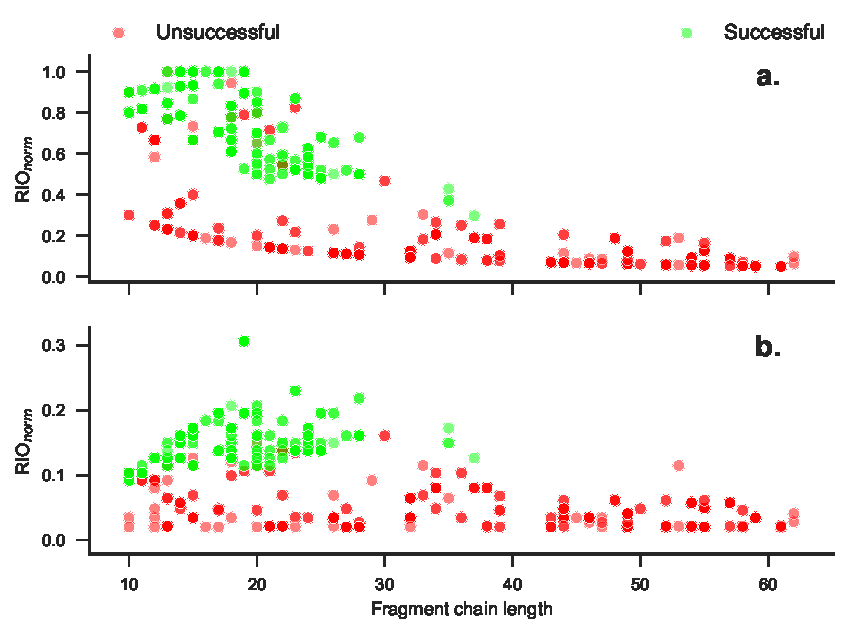
\includegraphics[width=\textwidth]{ample_flib_mrrionorm.pdf}
	\caption[Relationship between fragment chain length and normalised RIO scores.]{Dependence of normalised \acrlong{rio} (RIO\textsubscript{norm}) score on the fragment chain length. The two plots show  \gls{rio} scores normalised by the chain lengths of (a) the fragment and (b) the target. Colour coding indicates if the FLIB-fragment search model resulted in a structure solution. Each plot contains 1,780 fragment points.}
	\label{fig:ample_flib_mrrionorm}
\end{figure}

Sixty-six FLIB fragment have $>60$\% of their residues placed correctly yet did not lead to structure solution. These fragments were picked for the target sequences of T4 glutaredoxin (\gls{pdb} ID: 1aba) and 
4-hydroxybenzoyl CoA thioesterase (\gls{pdb} ID: 1lo7), and contain between 10 and 23 amino acids. These 66 fragments were derived from 15 targets and contain 17 unique peptide sequences. The fragments' \gls{rmsd} values are in range [0.19 2.72)\AA\ with a mean \gls{rmsd} of 1.10\AA. Surprisingly, almost all of these fragments contain primarily \textalpha-helices.


\section{Discussion}
The main objective of this study was to investigate the application of FLIB fragments to \gls{mr}.
